\chapter{Software Requirements Specification}
	Das Software Requirements Specification, kurz SRS, ist ein veröffentlichter Standard zur Spezifikation einer Software. Die Struktur eines SRS ist vom Institute of Electrical and Electronics Engineers im Standard IEEE 830-1998 festgehalten.
	
\section{Einführung}
	Das erste Unterkapitel des SRS erhält eine Beschreibung und eine Übersicht über alles, was im SRS enthalten ist.
	
	\subsection{Zweck}	
		Das SRS beschreibt den Projektumfang und die Anforderungen an die Software NoRPG. Es illustriert den Zweck und die vollständige Erklärung für die Entwicklung der Software. Dabei wird es auch Systemeinschränkungen, Schnittstellen und Interaktionen mit externen Schnittstellen erklären\footnote{vgl. Tripp \cite{srsIEEE}(1998) Seite 3}. 
	
		Die Zielgruppe des SRSs sind zunächst alle, die in irgendeiner Verbindung mit der Software stehen oder jene, die Interesse an der Umsetzung haben. Zudem dient die Spezifikation zur Kommunikation zwischen Stakeholder und Entwickler.
		
	\subsection{Umfang}
		Dieses SRS handelt von dem Software Produkt NoRPG. Bei NoRPG handelt es sich um eine Gamifizierung einer Lernspielbibliothek für Android. NoRPG stellt unterschiedlichste Lernspiele bereit und ist dabei wie ein Rollenspiel aufgebaut und besitzt auch dieselben charakteristischen Eigenschaften eines Rollenspiels. Zu den charakteristischen Eigenschaften gehören, dass der Spielende in die Rollen realer Menschen, fiktiver Figuren, Tiere oder auch Gegenstände übernehmen\footnote{vgl. Warwitz & Rudolf \cite{rpgSinn} Seite 78ff.}.
		
		NoRPG richtet sich an Kinder und soll durch die Eigenschaften eines Rollenspiels die Spieler dazu anregen, weitere Lernspiele herunterzuladen und zu spielen. Im nächsten Kapitel werden unter anderem die Gedanken zur Gestaltung und weitere Ziele von NoRPG genauer betrachtet. %VIELLEICHT HIER NOCH BISSCHEN MEHR VORWEG NEHMEN
		
	\subsection{Übersicht}
		Der Rest des SRS enthält zwei weitere Kapitel. Das zweite Kapitel bietet einen Überblick über die Systemfunktionalität und die Systeminteraktion mit anderen Systemen. Dieses Kapitel stellt auch verschiedene Arten von Stakeholdern und deren Interaktion mit dem System vor. Darüber hinaus werden auch die Einschränkungen des Systems und die Annahmen über das Produkt erwähnt.
	
		Das letzten Kapitel des SRS enthält ausführlich die Anforderungsspezifikation und eine Beschreibung der unterschiedlichen Systemschnittstellen. Es werden verschiedene Spezifikationstechniken verwendet, um die Anforderungen für unterschiedliche Zielgruppen genau festzulegen.
	
		Die Struktur dieses Kapitels entspricht dem im Standard beschriebenen. Nicht benötigte Kapitel des SRS wurden nicht aufgenommen.
		
\section{Allgemeine Beschreibung}
	In diesem Unterkapitel werden die allgemeinen Faktoren, die das Produkt und seine Anforderungen betreffen, beschrieben. Dieses Kapitel behandelt nicht die spezifischen Anforderungen sondern stellt den Hintergrund für diese Anforderungen dar. 

	\subsection{Produktperspektive}
		In diesem Unterabschnitt des SRS wird das Produkt in unterschiedlichen Perspektiven mit verwandten Produkten betrachtet, denn bei NoRPG handelt es sich nicht um ein selbstständiges abgeschlossenes Projekt.
		
		Es wird zwischen verschiendenen Schnittstellentypen unterschieden. Beispielsweise gibt es System-, Benutzer-, Hardware- oder Softwareschnittstellen. 
		
		Systemschnittstellen: each system interface and identify the functionality of the software to accomplish the system
requirement and the interface description to match the system. Bei NoRPG gibt es keine Systemschnittstellen. (Oder etwa Android???)

		Benutzerschnittstellen: each interface between the software product and its users. Bei NoRPG ist es die Benutzeroberfläche/GUI, das Head up Display/HUD im Spiel.
		
		Hardwareschnittstellen: each interface between the software product and the hardware components of the system. This includes conÞguration characteristics. Bei NoRPG Smartphone und seine Komponenten (Touchscreen, Speaker, ...). Dann noch Datenbank
		
		Softwareschnittstellen: use of other required software products and interfaces with other application systems. Bei NoRPG Android, Google Play Store, ... Dann noch Datenbank

	\subsection{Produktfunktionen}
		This subsection of the SRS should provide a summary of the major functions that the software will perform. 
		
		The functions should be organized in a way that makes the list of functions understandable to the customer or to anyone else reading the document for the first time.
		
		Hauptfunktion anbieten von Lernspielen nach einem Standard (grobes Vorgehen vorgegeben)
		Spieler kann seinen erstellten Charakter durch die Spielwelt steuern. Im Spiel kann er mit Elementen interagieren. Je nach Element starten unterschiedliche Aktionen. Zum Beispiel die Interaktion mit einem Mensch startet eine Unterhaltung, wodurch der Spieler mehr über das Spiel und das Konzept herausfinden kann. Die Interaktion mit einer Verschlossenen Truhe zeigt die Lernspiele, die gespielt werden müssen um die Truhe zu öffnen. Die Interaktion mit einer Truhe nach dem Spielen des Lernspieles ermöglicht dem Spieler die Truhe zu öffnen und dann Collectables zu sammeln.
		
		Menüfunktionen, neben kleineren Funktionen wie Spieloptionen (Sprach-, Grafikeinstellungen, ...) gibt es die Möglichkeit den Lernfortschritt des Spielers zu betrachten. Lernfortschritt funktion erklären ...
		
		%Graifk wo die Funktionen in Beziehungen stehen
	
	\subsection{Benutzermerkmale}
		NoRPG hat zwei unterschiedliche Benutzertypen: Kinder und Administratoren.
	
		Grundsätzlich richtet sich die App NoRPG an Kinder, die keine Möglichkeit haben eine Schule zu besuchen. Jedoch werden keine Benutzergruppen, sei es Erwachsene oder Kinder die zusätzlich Lernen wollen, für diese App ausgeschlossen. Die Kinder sollte Erfahrung mit der Verwendung eines Smartphones, insbesondere mit Android-Systemen, haben. Dazu zählt die Bedienung der Android-Oberfläche und insbesondere die Bedienung des Google Play Stores. Da es sich bei den Benutzern in den meisten Fällen um Kinder handelt, sollten diese englische Texte lesen und verstehen können. Denn zum voranschreiten muss der Benutzer die Unterhaltungen mit NPC zum herunterladen von Spielen verstehen können um die richtige Aktion auszuwählen.
		
		Die Administratoren wollen die Daten analysieren und daraus Aktionen ableiten. z.B. viele Kinder aus Brasilien -> zusätzliche Sprache portugiesisch ... Dafür müssen die gespeicherten Informationen anonymisiert werden, die richtigen Daten erhoben werden, ...
			
	\subsection{Einschränkungen}
		Eine allgemeine Beschreibung der anderen Elemente, die die Entwickler und Spieler begrenzen.
		
		%Einschränkung Entwickler
		Entwickler müssen sich an regulatorische Richtlinien, wie beispielsweise die Datenschutzerklärung von Google oder das IT-Sicherheitsgesetz, halten.
				
		Da NoRPG sich an Kinder in bildungsfernen Ländern richtet, darf NoRPG keine hohen Hardwareressourcen anfordern. Als Maßstab wird das Smartphone Samsung Galaxy S4 genommen %HIER BEGRÜNDUNG WIESO DAS SMARTPHONE und QUELLE. 
		Das Samsung Galaxy S4 kostet 250€\footnote{Stand 04.01.2017 Quelle: sdaqdsa} und hat einen Quadcore?? mit 1,6GHz und 2GB RAM sowie 16GB internen Speicher. Es ist die Android Version 5.0 Lollipop standardmäßig von Samsung installiert.
		
		Schnittstellen anbieten, wenn eine Webapplikation für Administratoren entwickelt wird um Daten besser auszuwerten. Oder Schnittstellen für Spielentwickler. (Bestätigen, dass das Kind den Kurs erfolgreich abgeschlossen hat)
				
		Verfügbar- und Zuverlässigkeit: Spiel muss Offline spiel und -startbar sein. Das Spiel muss sicherstellen, dass ein Kurs vollständig absolviert wird, damit keine verfälschten Daten gesendet werden. 

		Daten der Spieler werden anonymisiert gespeichert um anschließend Analysen zu machen, um rauszufinden in welchen Ländern, Stadtteilen oder Gegenden die meisten Kinder aktiv sind. Daher sollten nur relevante und notwendige Informationen gespeichert werden um diese dann analysieren zu können.
		
		%Einschränkung Spieler
		Internet zum Downloaden von Spielen, von NoRPG, installieren von Updates, Synchronisieren, Registrieren, Einloggen, Ausloggen (da Synchronisiert wird) 
		
		Genügend Speicherplatz, RAM und andere Ressourcen
				
	\subsection{Annahmen und Abhängigkeiten}
		Eine Annahme von NoRPG ist, dass es immer auf Smartphones, die genügend Leistung haben, verwendet wird. Wenn das Telefon nicht über genügend Hardwareressourcen für die Anwendung verfügt, kann es Szenarien geben, in denen die Anwendung nicht wie beabsichtigt oder überhaupt nicht funktioniert.
		
		Eine weitere Annahme ist, dass das Smartphone und dessen Hardware sowie Software funktionieren. Das Smartphone muss sich mit dem Internet verbinden können, wenn der Benutzer sich anmelden möchte oder Lernspiele herunterladen will. Neben einer funktionierenden Internetverbindung sollten andere Hardwareelemente wie die Lautsprecher oder der Touchscreen funktionieren. Das Smartphone muss eine gültige Android Version mit einem Google Konto besitzen.
		
	\subsection{Aufteilung der Anforderungen}
		In dem Fall, dass das Projekt verzögert wird, gibt es einige Anforderungen, die auf die nächste Version der Anwendung übertragen werden könnten.

\section{Spezifische Anforderungen}
	Das letzte Kapitel des SRS dient dazu alle Softwareanforderungen detailliert zu beschreiben. Dies ermöglicht es Designern ein System zu entwickeln, welches allen Anforderungen entspricht, und Testern das System ausreichend zu testen.
	
	\subsection{Externe Schnittstellen}
		Dieser Abschnitt ist die detaillierte Beschreibung aller Ein- und Ausgänge von NoRPG. Die Beschreibung ergänzt und vervollständigt die Schnittstellenbeschreibung von Kapitel 2.2.1. 
	
	%It should include both content and format as follows:
	%	a) Name;
	%	b) Beschreibung Zweck;
	%	c) Quelle des Inputs und Ziele des Outputs;
	%	d) Gültigkeitsbereich, Genauigkeit + Toleranz;
	%	e) Maßeinheit;
	%	f) Timing;
	%	g) Beziehungne zu anderen In-/Outputs;
	%	h) Screen(Bildschirm)format /-organisation;
	%	i) Fenster(Window)format /-organisation;
	%	j) Datenforrmat;
	%	k) Kommandoformat;
	%	l) End messages.
		
		\subsubsection{Benutzerschnittstellen}
			Die Benutzerschnittstellen, die user interfaces, sind der Punkt, an dem der Benutzer mit der Software interagiert. Zur Beschreibung der Benutzerschnittstellen werden logische Eigenschaften sowie Aspekte zur Optimierung formuliert.
			
			Einem Benutzer, der NoRPG zum ersten Mal startet oder der nicht angemeldet ist, wird der Login-Screen präsentiert. Auf dem Login-Screen hat der Benutzer die Möglichkeit sich mit seinem Benutzernamen und seinem Passwort anzumelden oder sich, falls noch nicht geschehen, bei NoRPG zu registrieren. Das Smartphone muss Quer gehalten werden, da alle Elemente des Bildschirms vertikal angeordnet sind. Diese Eigenschaft trifft auch auf alle anderen Benutzerschnittstellen zu. Das Layout des Login-Screens ist ein Border-Pane, in dem die Bestandteile in einer einzigen Spalte angeordnet sind. Zur Optimierung der Nutzung werden kurze Fehlermeldungen ausgegeben, wenn der Benutzer falsche Login-Daten eingibt.
			\begin{center}
				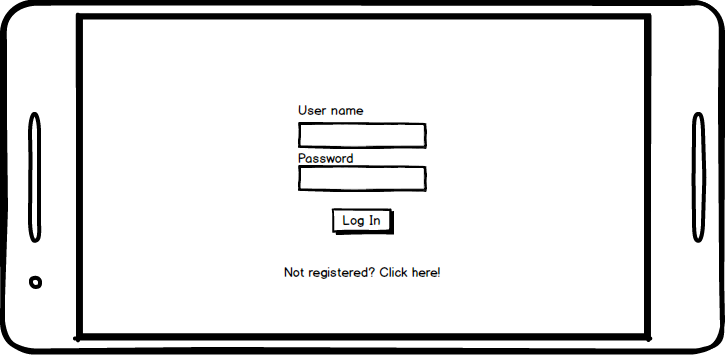
\includegraphics[width=10cm]{pics/Login_Mockup.png}
				\captionof{figure}{Login-Screen Mockup} 
			\end{center}
			
			Falls sich der Benutzer bei NoRPG registrieren möchte, hat er die Möglichkeit dies in der App zu machen. Dazu klickt der Benutzer im Login-Screen auf den Register-Button. Anschließend öffnet sich der Register-Screen. Die Elemente sind im Tabellen Layout angeordnet, wodurch der Benutzer weiß, welche Daten in welches Feld eingetragen werden müssen. Die Registrierung ist notwendig, damit der Spielstand, somit der Fortschritt in einer Relation mit dem Benutzer steht. Zur weiteren Optimierung werden kurze Fehlermeldungen ausgegeben, damit ich der Benutzer weiß, in welchem Feld ein Fehler ist.
			
			\begin{center}
				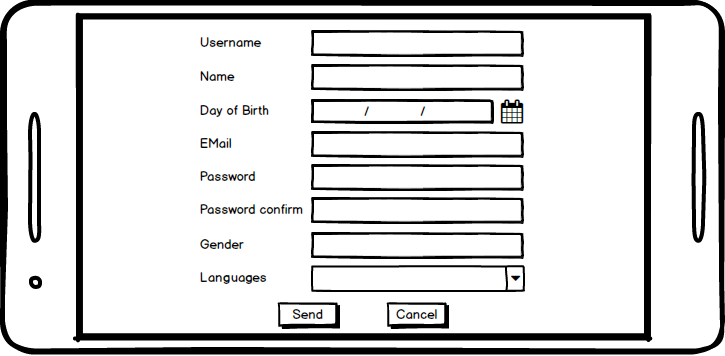
\includegraphics[width=10cm]{pics/Register_Mockup.png}
				\captionof{figure}{Register-Screen Mockup} 
			\end{center}
			
			Nach der Registrierung kann der Spieler einmalig seinen Charakter für den angelegten Account erstellen. Dazu bestimmt der Benutzer den Namen, das Geschlecht und das Aussehen des Charakters.
			
			\begin{center}
				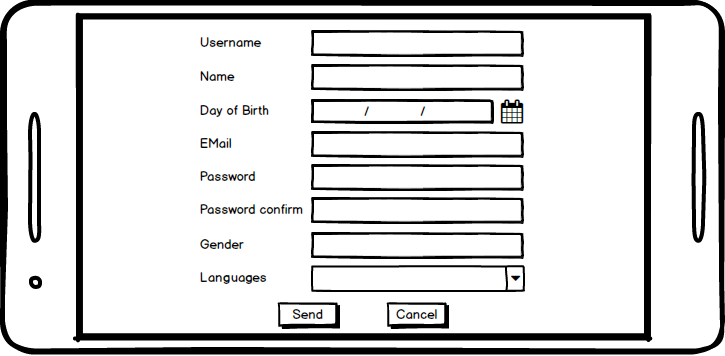
\includegraphics[width=10cm]{pics/Register_Mockup.png}
				\captionof{figure}{Register-Screen Mockup} 
			\end{center}
			
			NoRPG startet, nachdem alles geladen wurde und der Benutzer angemeldet ist. Das Spiele-Screen besteht aus der Spielewelt (Grafik) und dem Head-Up Display, kurz HUD. Das HUD ist eine Methode, mit der Informationen visuell als Teil der Benutzeroberfläche eines Spiels vermittelt werden. Während die Informationen, die auf dem HUD angezeigt werden, stark vom Spiel abhängen, gibt es viele Eigenschaften, die Spieler über viele Spiele erkennen. Die meisten von ihnen sind statisch auf dem Bildschirm, so dass sie während des Spiels sichtbar bleiben. 
			
			\begin{center}
				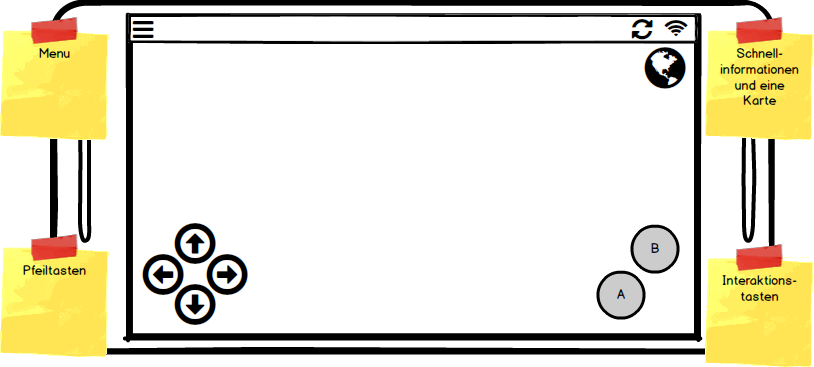
\includegraphics[width=11cm]{pics/HUD_Mockup.png}
				\captionof{figure}{HUD Mockup} 
			\end{center}
			
			Das Mockup 3 enthält alle direkt sichtbaren HUD Elemente, die während des Spieles aktiv sind. Die Elemente sind an die Ecken gebunden, so befindeen sich beispielsweise die Pfeiltasten zur Bewegung des Charakters in der linken unteren Ecke des Bildschirms (siehe Graifk). Es sind so wenig Elemente wie möglich auf dem Bildschirm angeordnet und die verwendeten Symbole sind aus anderen bekannten Spielen und Konsolen übernommen und sind quasi ein Standard. Durch diese bekannte Anordnung der Elemente kann der User Informationen schneller verstehen und schneller reagieren. %vllt bisschen noch was zu dieser Anordnung labern
			
			Das Menü, welches sich in der oberen linken Ecke befindet, kann geöffnet werden. Dadurch wird das laufende Spiel pausiert und es werden weitere Optionen bzw. Interaktionen mit dem Spiel möglich. Diese HUD Elemente werden nur dann sichtbar, wenn der Spieler das Menü öffnet. Dadurch rückt das Spiel und die anderen Elemente in den Hintergrund. Das bedeutet nicht, dass die Elemente ausgeblendet werden, sondern dass der Benutzer diese Elemente nicht benutzen kann solange das Menü offen ist.
			
			\begin{center}
				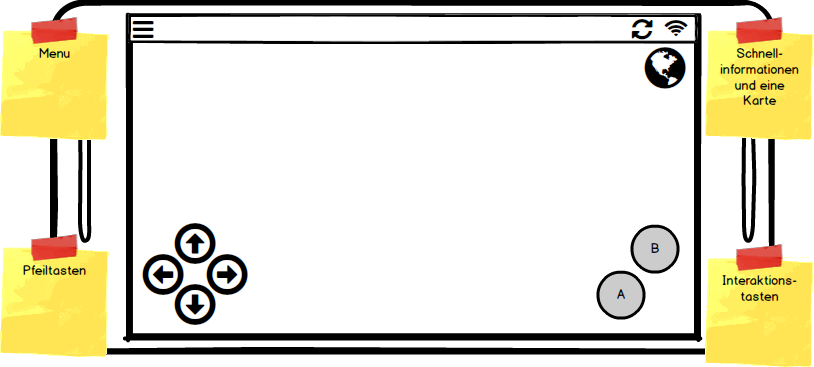
\includegraphics[width=11cm]{pics/HUD_Mockup.png}
				\captionof{figure}{HUD offenes Menü Mockup} 
			\end{center}
			
			Einige der Menü-Elemente öffnen wiederum einen anderen Screen. Diese werden dann über das aktuelle Spiel geöffnet. Das Spiel befindet sich im Hintergrund und kann nicht gesehen bzw. angeklickt werden. Der neu geöffnete Screen muss erst geschlossen werden um das Spiel fortsetzen zu können. Ein Beispiel dafür ist der Fortschritt-Screen. Hier kann der Benutzer seinen Lern- bzw. Spielfortschritt betrachten.
			
			\begin{center}
				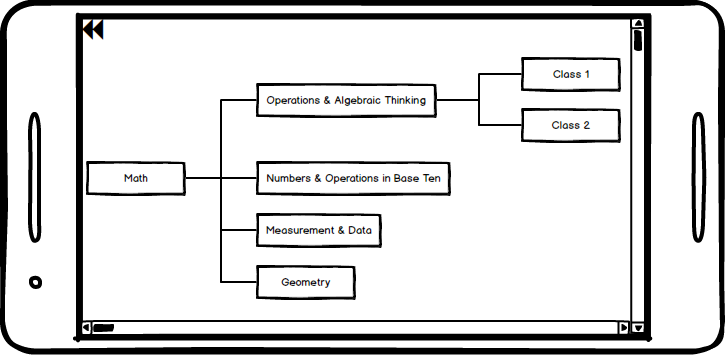
\includegraphics[width=10cm]{pics/Fortschritt_Mockup.png}
				\captionof{figure}{Fortschritt-Screen Mockup} 
			\end{center}
			
			Die Auflistung aller Screens würde den Rahmen dieser Arbeit überschreiten. Daher befinden sich die Mockups für die restlichen Screens im Anhang.
						
			%logische Eigenschaften:  required screen formats, page or window layouts, content of any reports or menus, or availability of programmable function keys
			
			%Aspekte Optimierung: comprise a list of do's and don'ts on how the system will appear to the user: long or short error messages
		
		\subsubsection{Hardwareschnittstellen}
			Die Hardwareschnittstellen spezifiziert die logischen Eigenschaften jeder Schnittstelle zwischen NoRPG und den Hardwarekomponenten des Systems.
			
			NoRPG besitzt keine direkten Hardwareschnittstellen: Verbunden mit Lautsprechern für Soundausgaben, Touchscreen für Eingaben/Interaktionen, WLAN für die Verbindung mit dem Server/Synchronisierung, Verbindung zum Datenbank Server
			
		\subsubsection{Softwareschnittstellen}
			This should specify the use of other required software products and interfaces with other application systems 
			
			Data mangement system, Android OS

	\subsection{Funktionale Anforderungen}
		Use Cases dokumentieren Funktionalitäten eines Systems auf Basis von einfachen Modellen. In einem Use Case wird das nach außen sichtbare Verhalten eines Systems aus der Sicht der Nutzer beschrieben. Ein Nutzer kann hierbei eine Person, eine Rolle oder ein anderes System sein. Dieser Nutzer tritt als Akteur mit dem System in Interaktion, um ein bestimmtes Ziel zu erreichen.
	
		\begin{center}
			
\includegraphics[width=\textwidth]{pics/OUCD.pdf}
			\captionof{figure}{Overall Use Case Diagramm} 
		\end{center}
	
		In der Grafik sind 2 Systeme zu sehen. Links das vorhandene System Hone welches ein Frontend für die Entwickler und für die Kinder darstellt. Die Kinder sollen nicht mehr über Hone die Spiele herunterladen sondern nur noch die App NoRPG verwenden. Die Ansicht wird jedoch weiterhin genutzt und soll den Eltern der Kinder die Möglichkeit geben, den Fortschritt des Kindes nachzuschauen. Hone soll von den Rollen Entwickler und Eltern entwickelt werden.
	
		Das rechte System NoRPG stellt die zu entwickelnde App dar. Diese dient als Frontend für das Kind. Es gibt viele Use Cases. Die Use Cases werden in unterschiedliche Gruppen zusammengefasst. Die nächsten Unterkapitel sind die einzelnen Gruppierungen.
	
		\subsubsection{Login}
			Dieser Use Case beschreibt den Anwendungsfall, dass der Benutzer sich bei NoRPG anmelden möchte. Eine Anmeldung ist notwendig um NORPG zu starten. Die Besonderheit bei der Anmeldung  ist, dass der Account des Benutzers auch für die Anmeldung bei Hone benötigt wird. Der Benutzer kann sich in NoRPG im Startbildschirm anmelden und anschließend das Spiel zu starten.
			
			\paragraph{Ereignisablauf}
				Eingeben von Benutzername und Passwort.	Klicke auf Login.
			
				Alternativer Ablauf: Abbruch oder Spiel Beenden
			
			\paragraph{Vorbedingungen}
				Benutzer ist registriert, Während der Anmeldung ist eine Internetverbindung vorhanden, Kombination von Benutzername und Passwort existiert, es ist kein anderer Benutzer auf dem Gerät angemeldet
			
			\paragraph{Nachbedingungen}
				Benutzer angemeldet, kann online oder offline weiterspielen. Beim nächsten Start der App ist der Benutzer automatisch angemeldet.
			
				Oder falls die eingegeben Daten nicht übereinstimmen, Fehlermeldung anzeigen
	
		\subsubsection{Create character}
			Dieser Use Case beschreibt den Anwendungsfall, dass der Benutzer seinen Charakter erstellen möchte. Dies ist eine einmalige Aktion, die beim ersten Anmelden durchlaufen wird. 
			
			\paragraph{Ereignisablauf}
				Wenn der Benutzer sich zum ersten mal anmeldet hat er die Möglichkeit seinen Charakter zu erstellen. Dafür wählt der Benutzer sich zunächst sein Geschlecht aus und wählt anschließend den passenden Charakter.
			
				Zum Abschluss vergibt der Benutzer seinen Charakter einen Namen.
	
			\paragraph{Vorbedingungen}
				Der Account meldet sich das erste mal in der App an.
			
			\paragraph{Nachbedingungen}
				Nach der Erstellung beginnt das Spiel und der Charakter ist gespeichert. Bei erneuter Anmeldung muss der Benutzer nicht erneut einen Charakter erstellen.
	
		\subsubsection{Player interaction}
			Dieser Use Case beschreibt den Anwendungsfall: Benutzer interaktionen, wie Bewegen oder Bestätigen.
			
			\paragraph{Ereignisablauf}
				Klickt auf Pfeiltasten, Charakter bewegt sich in diese Richtung
			
				Klickt auf A, Charakter bestätigt
			
				Klickt auf B, Charakter lehnt ab
			
				(Bild Mockup)
			
			\paragraph{Vorbedingungen}
				Spieler befindet sich im Spiel (nicht loading screen und menü ist geschlossen)
			
			\paragraph{Nachbedingungen}
				Charakter bewegt sich, bestätigt oder lehnt ab
	
		\subsubsection{NPC interaction}
			Dieser Use Case beschreibt den Anwendungsfall, dass der Benutzer sich in einer Interaktion mit einem NPC befindet. NPC bedeutet Non-Player Charakter und stellt die programmierten Charaktere dar (Unterhaltungen mit NPC, Storytelling)
			
			\paragraph{Ereignisablauf}
				Ereignisablauf etc.

			\paragraph{Vorbedingungen}
				Ingame, nicht loading screen oder menü offen
			
			\paragraph{Nachbedingungen}
				Unterhaltung findet statt, etc.
	
		\subsubsection{Choose games}
			Dieser Use Case beschreibt den Anwendungsfall, dass der Benutzer ein spiel zum downloaden auswählt
			
			\paragraph{Ereignisablauf}
				Der Benutzer kann sich (wenn vorhanden) zwischen mehrere Spielen auswählen um den Kurs abzuschließen.

			\paragraph{Vorbedingungen}
				Internetverbindung, darf die SPiele nach dem Standard spielen
			
			\paragraph{Nachbedingungen}
				Weiterleitung auf Google Play Store

		\subsubsection{Open map}
			Dieser Use Case beschreibt den Anwendungsfall, dass der Benutzer die Karte öffnet. Die Karte dient zur Orientierung der Welt und beinhaltet Symbole etc. um herauszufinden was so ist
			
			\paragraph{Ereignisablauf}
			Benutzer öffnet Menü und klickt auf "Map" ...
	
			\paragraph{Vorbedingungen}
				Menü offen, Benutzer befindet sich nicht in einer NPC Interaktion
			
			\paragraph{Nachbedingungen}
				Eine Karte von der aktuellen Welt wird geöffnet
	
		\subsubsection{Show games}
			Dieser Use Case beschreibt den Anwendungsfall: Liste der gespielten und heruntergeladneen Spiele wird angezeigt. Zuordnung zu den Standards. Aus NoRPG das Spiel starten können.
			
			\paragraph{Ereignisablauf}
				Benuter öffnet Menü und klickt auf "Games" ...

			\paragraph{Vorbedingungen}
				Menü offen, Benutzer befindet sich nicht in einer NPC interaktion
			
			\paragraph{Nachbedingungen}
				Eine Liste wird angezeigt
	
		\subsubsection{View progress}
			Dieser Use Case beschreibt den Anwendungsfall, dass der Benutzer 
			
			\paragraph{Ereignisablauf}
	
			\paragraph{Vorbedingungen}
			
			\paragraph{Nachbedingungen}
	
		\subsubsection{Settings}
			Dieser Use Case beschreibt den Anwendungsfall, dass der Benutzer 
			
			\paragraph{Ereignisablauf}
	
			\paragraph{Vorbedingungen}
			
			\paragraph{Nachbedingungen}
	
		\subsubsection{Synchronize}
			Dieser Use Case beschreibt den Anwendungsfall, dass der Benutzer 
			
			\paragraph{Ereignisablauf}
	
			\paragraph{Vorbedingungen}
			
			\paragraph{Nachbedingungen}
	
		\subsubsection{Save local}
			Dieser Use Case beschreibt den Anwendungsfall, dass der Benutzer 
			
			\paragraph{Ereignisablauf}
	
			\paragraph{Vorbedingungen}
			
			\paragraph{Nachbedingungen}
	
	\subsection{Performanz Anforderungen}
		This subsection should specify both the static and the dynamic numerical requirements placed on the software or on human interaction with the software as a whole. Static numerical requirements may include the following
		
		The number of terminals to be supported, The number of simultaneous users to be supported, Amount and type of information to be handled
		
	\subsection{Datenbank Anforderungen}
		This should specify the logical requirements for any information that is to be placed into a database. This may include the following:
		
		Types of information used by various functions
		
		Frequency of use
		
		Accessing capabilities
		
		Data entities and their relationships
		
		Integrity constraints
		
		Data retention requirements.
	
	\subsection{Entwurfsbeschränkungen}
		This should specify design constraints that can be imposed by other standards, hardware limitations, etc.
		
		Standards compliance: This subsection should specify the requirements derived from existing standards or regulations. They may include the following: 
		
		Report format, Data naming, Accounting procedures and Audit tracing.
	
	\subsection{Benuzterfreundlichkeit}

	\subsection{Zuverlässigkeit}
		This should specify the factors required to establish the required reliability of the software system at time of delivery.
	
	\subsection{Verfügbarkeit}
		This should specify the factors required to guarantee a deÞned availability level for the entire system such as checkpoint, recovery, and restart. 
	
	\subsection{Sicherheit}
		This should specify the factors that protect the software from accidental or malicious access, use, modiÞcation, destruction, or disclosure. SpeciÞc requirements in this area could include the need to
		
		Utilize certain cryptographical techniques; 
		
		Keep speciÞc log or history data sets;
		
		Assign certain functions to different modules;
		
		Restrict communications between some areas of the program;
		
		Check data integrity for critical variables.
	
	\subsection{Wartbarkeit}
		This should specify attributes of software that relate to the ease of maintenance of the software itself. There may be some requirement for certain modularity, interfaces, complexity, etc. Requirements should not be placed here just because they are thought to be good design practices.
	
	\subsection{Portabilität}
		This should specify attributes of software that relate to the ease of porting the software to other host machines and/or operating systems. This may include the following:
		
		Percentage of components with host-dependent code;
		
		Percentage of code that is host dependent;
		
		Use of a proven portable language; 
		
		Use of a particular compiler or language subset;
		
		Use of a particular operating system.
